\section{Intregación por sustitución trigonométrica}
Para resolver estas integrales es necesario conocer o tomar como medida de apoyo un triangulo rectangulo, el cual nos facilitara en realizar un cambio de variable al momento de realizar una integral.\\

\subsection{Caso I}

\begin{center}
  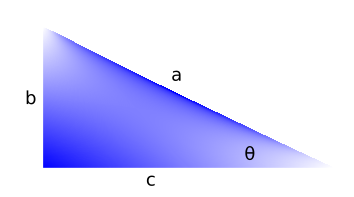
\includegraphics[scale=0.5]{imgsAux/triangulo.png}\\
\end{center}

Donde:

\begin{equation*}
    \begin{gathered}
        a=a, \;\;\; b=x \;\;\;\&\;\;\; c=\sqrt{a^{2}-x^{2}}
    \end{gathered}
\end{equation*}

Partiendo de esto obtendremos:

\begin{equation*}
    \begin{gathered}
        \sin(\theta)= \frac{x}{a},\;\;\; x=a\sin(\theta),\;\;\; dx=a\cos(\theta)d\theta
    \end{gathered}
\end{equation*}
% Ecuación 1 %
% \(\displaystyle \) %
Con ello sustituyendo a \(\displaystyle x\) tendremos:

\begin{equation*}
    \begin{gathered}
        \sqrt{a^{2}-x^{2}}\Rightarrow \sqrt{a^{2}-a^{2}\sin^{2}(\theta)} \Leftrightarrow \sqrt{a^{2}[1-\sin^{2}(\theta)]} \Leftrightarrow \sqrt{a^{2}\cos^{2}(\theta)}\;\;\;\;\; \therefore \sqrt{a^{2}-x^{2}}=a\cos(\theta)
    \end{gathered}
\end{equation*}

\subsection{Caso II}

\begin{center}
  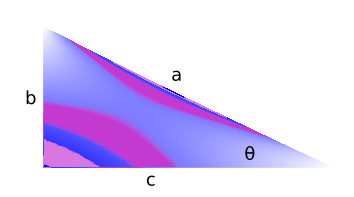
\includegraphics[scale=0.5]{imgsAux/triangulo1.png}\\
\end{center}

Donde:

\begin{equation*}
    \begin{gathered}
        a=\sqrt{a^{2}+x^{2}}\;\;\;, b=x \;\;\;\&\;\;\; c=a
    \end{gathered}
\end{equation*}

Partiendo de esto obtendremos:

\begin{equation*}
    \begin{gathered}
        \tan(\theta)= \frac{x}{a},\;\;\; x=a\tan(\theta),\;\;\; dx=a\sec^{2}(\theta)d\theta
    \end{gathered}
\end{equation*}

Con ello sustituyendo a \(\displaystyle x\) tendremos:

\begin{equation*}
    \begin{gathered}
        \sqrt{a^{2}+x^{2}}\Rightarrow \sqrt{a^{2}+a^{2}\tan^{2}(\theta)} \Leftrightarrow \sqrt{a^{2}[1+\tan^{2}(\theta)]} \Leftrightarrow \sqrt{a^{2}\sec^{2}(\theta)}\;\;\;\;\; \therefore \sqrt{a^{2}+x^{2}}=a\sec(\theta)
    \end{gathered}
\end{equation*}

\clearpage
\subsection{Caso III}

\begin{center}
  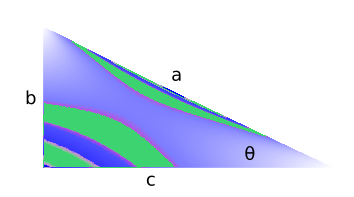
\includegraphics[scale=0.5]{imgsAux/triangulo2.png}\\
\end{center}

Donde:

\begin{equation*}
    \begin{gathered}
        a=x,\;\;\; b=\sqrt{x^{2}-a^{2}} \;\;\;\&\;\;\; c=a
    \end{gathered}
\end{equation*}

Partiendo de esto obtendremos:

\begin{equation*}
    \begin{gathered}
        \sec(\theta)= \frac{x}{a},\;\;\; x=a\sec(\theta),\;\;\; dx=a\sec(\theta)\tan(\theta)d\theta
    \end{gathered}
\end{equation*}

Con ello sustituyendo a \(\displaystyle x\) tendremos:

\begin{equation*}
    \begin{gathered}
        \sqrt{x^{2}-a^{2}}\Rightarrow \sqrt{a^{2}\sec^{2}(\theta)-a^{2}} \Leftrightarrow \sqrt{a^{2}[\sec^{2}(\theta)-1]} \Leftrightarrow \sqrt{a^{2}\tan^{2}(\theta)}\;\;\;\;\; \therefore \sqrt{x^{2}-a^{2}}=a\tan(\theta)
    \end{gathered}
\end{equation*}

\textit{\textbf{Aplicado ahora en alguna integral tendremos:}}
% Ecuación 1 %
% \(\displaystyle \) %
\begin{equation}
    \begin{gathered}
        \int \frac{dx}{\sqrt{9+x^{2}}}
    \end{gathered}
\end{equation}

\textit{Solución}\\

De acuerdo con los casos que tenemos podemos aplicar el Caso II en el problema por lo que sustituyendo directamente tendremos \(\displaystyle a=3\) \& \(\displaystyle x=3\tan(\theta)\):

\begin{equation*}
    \begin{gathered}
        \int \frac{3\sec^{2}(\theta)}{3\sec(\theta)}d\theta \; \Leftrightarrow \; \int \sec(\theta)d\theta = \ln\left|\sec(\theta)+\tan(\theta)\right|+C
    \end{gathered}
\end{equation*}

Finalmente sustituiremos los valores de las identidades trigonométricas con sus respectivos valores de triangulo:

\begin{equation*}
    \begin{gathered}
        \int \frac{dx}{\sqrt{9+x^{2}}}= \ln\left|\frac{\sqrt{9+x^{2}}}{3}+\frac{x}{3}\right|+C
    \end{gathered}
\end{equation*}

\vspace{1cm}

\begin{equation}
    \begin{gathered}
        \int\frac{dx}{\sqrt{x^{2}+2x+26}}
    \end{gathered}
\end{equation}

\textit{Solución}\\

Para abordar este problema a traves de sustitución trigonométrica es necesario reducir el polinomio interno de la raíz cuadrada, por lo primer rescribiremos la integral:

\begin{equation*}
    \begin{gathered}
        \int \frac{dx}{\sqrt{x^{2}+2x+25+1}}\Leftrightarrow \int \frac{dx}{\sqrt{(x+1)^{2}+5^{2}}}
    \end{gathered}
\end{equation*}

Ahora una vez reduciendo esto haremos un cambio de variable el cual sera \(\displaystyle u=x+1\) \& \(\displaystyle du=dx\), reescribiendo la integral tenemos:

\begin{equation*}
    \begin{gathered}
        \int \frac{du}{\sqrt{u^{2}+5^{2}}}
    \end{gathered}
\end{equation*}

Con esto podemos aplicar directamente el Caso II, por lo que saltando todo el cambio de variable hacia \(\displaystyle\theta\) debido al anterior ejemplo tendremos:

\begin{equation*}
    \begin{gathered}
        \int \frac{du}{\sqrt{u^{2}+5^{2}}}=\ln\left|\sec(\theta)+\tan(\theta)\right|+C
    \end{gathered}
\end{equation*}

Lo cual es:

\begin{equation*}
    \begin{gathered}
        \int \frac{du}{\sqrt{u^{2}+5^{2}}}=\ln\left|\frac{\sqrt{u^{2}+25}}{5}+\frac{u}{5}\right|+C
    \end{gathered}
\end{equation*}

Sustituyendo el valor de \(\displaystyle u\) por su respectivo valor en \(\displaystyle x\):

\begin{equation*}
    \begin{gathered}
        \int\frac{dx}{\sqrt{x^{2}+2x+26}}=\ln\left|\frac{{\sqrt{(x+1)^2+25}}}{5}+\frac{x+1}{5}\right|+C
    \end{gathered}
\end{equation*}
\textbf{Ejercicio propuesto:}
\begin{enumerate}
  \item \(\displaystyle\int\frac{\sqrt{x^{2}-4}}{x}dx\)
\end{enumerate}
\clearpage